\documentclass{standalone}
\usepackage{tikz}
\usetikzlibrary{patterns, positioning}


\begin{document}
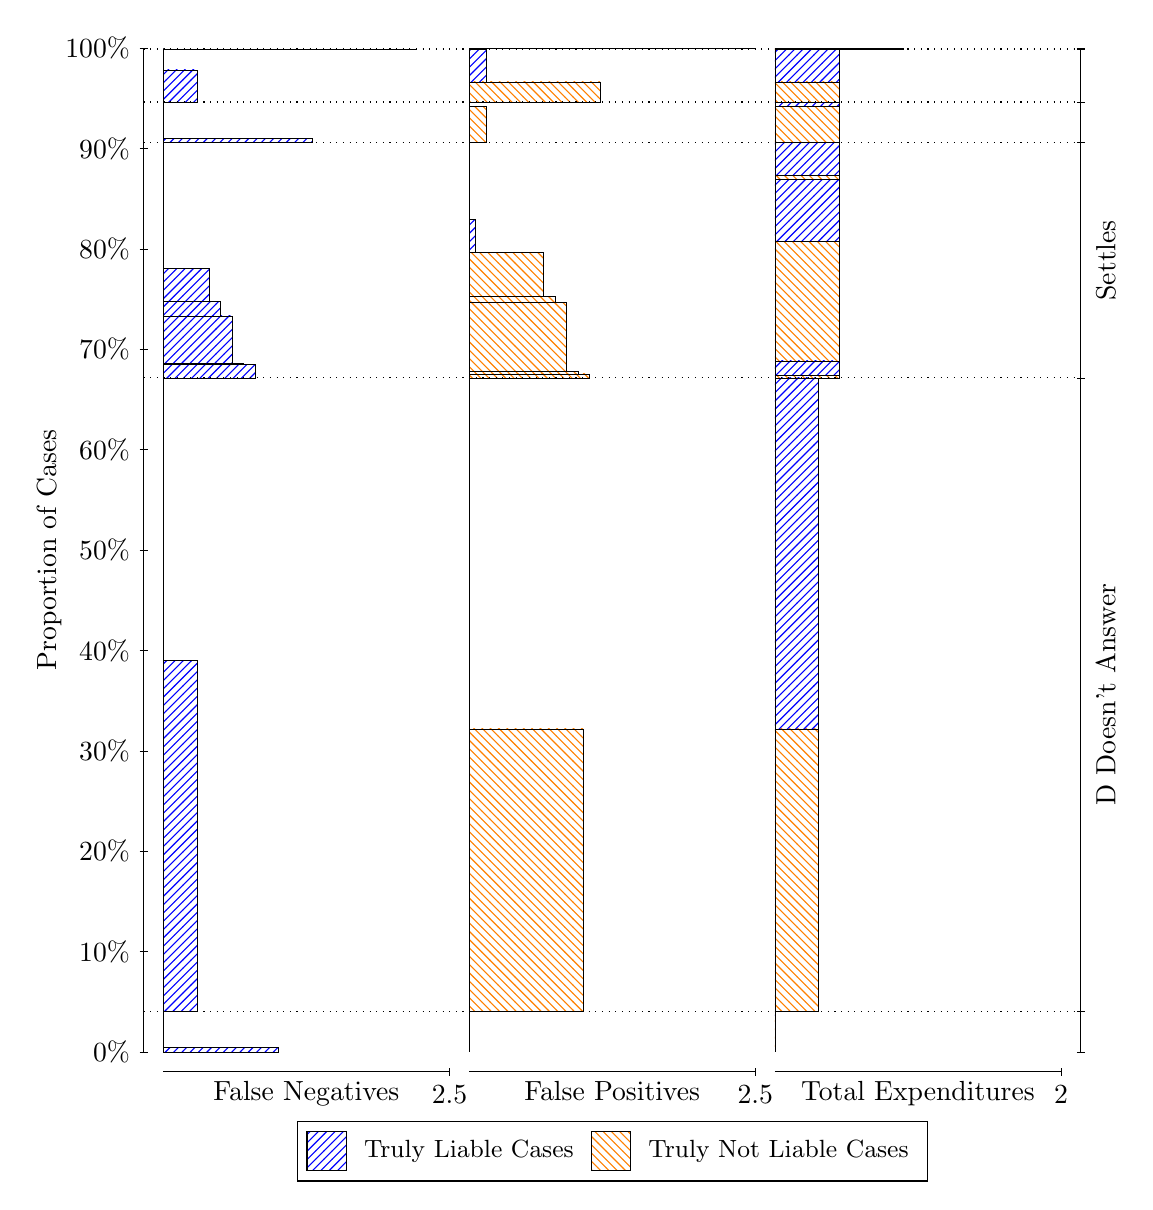
\begin{tikzpicture}
\draw[black, very thin] (1.5,1.75) -- (1.5,14.5);
\node[rotate=90, text=black, anchor=center] at (0.3, 8.125) {Proportion of Cases};
\draw[black, very thin] (1.45,1.75) -- (1.55,1.75);
\node[text=black, anchor=east] at (1.45, 1.75) {0\%};
\draw[black, very thin] (1.45,3.025) -- (1.55,3.025);
\node[text=black, anchor=east] at (1.45, 3.025) {10\%};
\draw[black, very thin] (1.45,4.3) -- (1.55,4.3);
\node[text=black, anchor=east] at (1.45, 4.3) {20\%};
\draw[black, very thin] (1.45,5.575) -- (1.55,5.575);
\node[text=black, anchor=east] at (1.45, 5.575) {30\%};
\draw[black, very thin] (1.45,6.85) -- (1.55,6.85);
\node[text=black, anchor=east] at (1.45, 6.85) {40\%};
\draw[black, very thin] (1.45,8.125) -- (1.55,8.125);
\node[text=black, anchor=east] at (1.45, 8.125) {50\%};
\draw[black, very thin] (1.45,9.4) -- (1.55,9.4);
\node[text=black, anchor=east] at (1.45, 9.4) {60\%};
\draw[black, very thin] (1.45,10.675) -- (1.55,10.675);
\node[text=black, anchor=east] at (1.45, 10.675) {70\%};
\draw[black, very thin] (1.45,11.95) -- (1.55,11.95);
\node[text=black, anchor=east] at (1.45, 11.95) {80\%};
\draw[black, very thin] (1.45,13.225) -- (1.55,13.225);
\node[text=black, anchor=east] at (1.45, 13.225) {90\%};
\draw[black, very thin] (1.45,14.5) -- (1.55,14.5);
\node[text=black, anchor=east] at (1.45, 14.5) {100\%};

\draw[black, very thin] (13.4,1.75) -- (13.4,14.5);
\draw[black, very thin] (13.35,1.75) -- (13.45,1.75);
\node[anchor=west] at (13.35, 1.75) {};
\draw[black, very thin] (13.35,2.263) -- (13.45,2.263);
\node[anchor=west] at (13.35, 2.263) {};
\draw[black, very thin] (13.35,10.311) -- (13.45,10.311);
\node[anchor=west] at (13.35, 10.311) {};
\draw[black, very thin] (13.35,13.297) -- (13.45,13.297);
\node[anchor=west] at (13.35, 13.297) {};
\draw[black, very thin] (13.35,13.814) -- (13.45,13.814);
\node[anchor=west] at (13.35, 13.814) {};
\draw[black, very thin] (13.35,14.479) -- (13.45,14.479);
\node[anchor=west] at (13.35, 14.479) {};
\draw[black, very thin] (13.35,14.493) -- (13.45,14.493);
\node[anchor=west] at (13.35, 14.493) {};
\draw[black, very thin] (13.35,14.5) -- (13.45,14.5);
\node[anchor=west] at (13.35, 14.5) {};

\draw[black, very thin, pattern color=blue, pattern=north east lines] (1.75,1.75) rectangle (3.2033,1.804);
\draw[black, very thin, pattern color=orange, pattern=north west lines] (1.75,1.804) rectangle (1.75,2.263);
\draw[black, very thin, pattern color=blue, pattern=north east lines] (1.75,2.263) rectangle (2.186,6.7206);
\draw[black, very thin, pattern color=orange, pattern=north west lines] (1.75,6.7206) rectangle (1.75,10.311);
\draw[black, very thin, pattern color=blue, pattern=north east lines] (1.75,10.311) rectangle (2.9127,10.485);
\draw[black, very thin, pattern color=blue, pattern=north east lines] (1.75,10.485) rectangle (2.7673,10.492);
\draw[black, very thin, pattern color=blue, pattern=north east lines] (1.75,10.492) rectangle (2.622,11.097);
\draw[black, very thin, pattern color=blue, pattern=north east lines] (1.75,11.097) rectangle (2.4767,11.284);
\draw[black, very thin, pattern color=blue, pattern=north east lines] (1.75,11.284) rectangle (2.3313,11.7);
\draw[black, very thin, pattern color=orange, pattern=north west lines] (1.75,11.7) rectangle (1.75,13.297);
\draw[black, very thin, pattern color=blue, pattern=north east lines] (1.75,13.297) rectangle (3.6393,13.354);
\draw[black, very thin, pattern color=orange, pattern=north west lines] (1.75,13.354) rectangle (1.75,13.814);
\draw[black, very thin, pattern color=blue, pattern=north east lines] (1.75,13.814) rectangle (2.186,14.223);
\draw[black, very thin, pattern color=orange, pattern=north west lines] (1.75,14.223) rectangle (1.75,14.479);
\draw[black, very thin, pattern color=blue, pattern=north east lines] (1.75,14.479) rectangle (4.9473,14.483);
\draw[black, very thin, pattern color=orange, pattern=north west lines] (1.75,14.483) rectangle (1.75,14.493);
\draw[black, very thin, pattern color=orange, pattern=north west lines] (1.75,14.493) rectangle (1.75,14.496);
\draw[black, very thin, pattern color=blue, pattern=north east lines] (1.75,14.496) rectangle (1.75,14.5);
\draw[black, very thin, pattern color=orange, pattern=north west lines] (5.6333,1.75) rectangle (5.6333,2.2091);
\draw[black, very thin, pattern color=blue, pattern=north east lines] (5.6333,2.2091) rectangle (5.6333,2.263);
\draw[black, very thin, pattern color=orange, pattern=north west lines] (5.6333,2.263) rectangle (7.0867,5.8533);
\draw[black, very thin, pattern color=blue, pattern=north east lines] (5.6333,5.8533) rectangle (5.6333,10.311);
\draw[black, very thin, pattern color=orange, pattern=north west lines] (5.6333,10.311) rectangle (7.1593,10.362);
\draw[black, very thin, pattern color=orange, pattern=north west lines] (5.6333,10.362) rectangle (7.014,10.391);
\draw[black, very thin, pattern color=orange, pattern=north west lines] (5.6333,10.391) rectangle (6.8687,11.267);
\draw[black, very thin, pattern color=orange, pattern=north west lines] (5.6333,11.267) rectangle (6.7233,11.346);
\draw[black, very thin, pattern color=orange, pattern=north west lines] (5.6333,11.346) rectangle (6.578,11.907);
\draw[black, very thin, pattern color=blue, pattern=north east lines] (5.6333,11.907) rectangle (5.706,12.323);
\draw[black, very thin, pattern color=blue, pattern=north east lines] (5.6333,12.323) rectangle (5.6333,13.297);
\draw[black, very thin, pattern color=orange, pattern=north west lines] (5.6333,13.297) rectangle (5.8513,13.756);
\draw[black, very thin, pattern color=blue, pattern=north east lines] (5.6333,13.756) rectangle (5.6333,13.814);
\draw[black, very thin, pattern color=orange, pattern=north west lines] (5.6333,13.814) rectangle (7.3047,14.07);
\draw[black, very thin, pattern color=blue, pattern=north east lines] (5.6333,14.07) rectangle (5.8513,14.479);
\draw[black, very thin, pattern color=orange, pattern=north west lines] (5.6333,14.479) rectangle (5.6333,14.49);
\draw[black, very thin, pattern color=blue, pattern=north east lines] (5.6333,14.49) rectangle (5.6333,14.493);
\draw[black, very thin, pattern color=orange, pattern=north west lines] (5.6333,14.493) rectangle (9.2667,14.496);
\draw[black, very thin, pattern color=blue, pattern=north east lines] (5.6333,14.496) rectangle (7.8133,14.5);
\draw[black, very thin, pattern color=orange, pattern=north west lines] (9.5167,1.75) rectangle (9.5167,2.2091);
\draw[black, very thin, pattern color=blue, pattern=north east lines] (9.5167,2.2091) rectangle (9.5167,2.263);
\draw[black, very thin, pattern color=orange, pattern=north west lines] (9.5167,2.263) rectangle (10.062,5.8533);
\draw[black, very thin, pattern color=blue, pattern=north east lines] (9.5167,5.8533) rectangle (10.062,10.311);
\draw[black, very thin, pattern color=orange, pattern=north west lines] (9.5167,10.311) rectangle (10.334,10.34);
\draw[black, very thin, pattern color=blue, pattern=north east lines] (9.5167,10.34) rectangle (10.334,10.528);
\draw[black, very thin, pattern color=orange, pattern=north west lines] (9.5167,10.528) rectangle (10.334,12.044);
\draw[black, very thin, pattern color=blue, pattern=north east lines] (9.5167,12.044) rectangle (10.334,12.829);
\draw[black, very thin, pattern color=orange, pattern=north west lines] (9.5167,12.829) rectangle (10.334,12.88);
\draw[black, very thin, pattern color=blue, pattern=north east lines] (9.5167,12.88) rectangle (10.334,13.297);
\draw[black, very thin, pattern color=orange, pattern=north west lines] (9.5167,13.297) rectangle (10.334,13.756);
\draw[black, very thin, pattern color=blue, pattern=north east lines] (9.5167,13.756) rectangle (10.334,13.814);
\draw[black, very thin, pattern color=orange, pattern=north west lines] (9.5167,13.814) rectangle (10.334,14.07);
\draw[black, very thin, pattern color=blue, pattern=north east lines] (9.5167,14.07) rectangle (10.334,14.479);
\draw[black, very thin, pattern color=orange, pattern=north west lines] (9.5167,14.479) rectangle (11.152,14.49);
\draw[black, very thin, pattern color=blue, pattern=north east lines] (9.5167,14.49) rectangle (11.152,14.493);
\draw[black, very thin, pattern color=orange, pattern=north west lines] (9.5167,14.493) rectangle (11.152,14.496);
\draw[black, very thin, pattern color=blue, pattern=north east lines] (9.5167,14.496) rectangle (11.152,14.5);
\draw[black, dotted] (1.5,2.263) -- (13.4,2.263);
\draw[black, dotted] (1.5,10.311) -- (13.4,10.311);
\draw[black, dotted] (1.5,13.297) -- (13.4,13.297);
\draw[black, dotted] (1.5,13.814) -- (13.4,13.814);
\draw[black, dotted] (1.5,14.479) -- (13.4,14.479);
\draw[black, dotted] (1.5,14.493) -- (13.4,14.493);
\draw[black, very thin] (1.75,1.5) -- (5.3833,1.5);
\node[text=black, anchor=north] at (3.5667, 1.5) {False Negatives};
\draw[black, very thin] (5.3833,1.45) -- (5.3833,1.55);
\node[text=black, anchor=north] at (5.3833, 1.45) {2.5};

\draw[black, very thin] (5.6333,1.5) -- (9.2667,1.5);
\node[text=black, anchor=north] at (7.45, 1.5) {False Positives};
\draw[black, very thin] (9.2667,1.45) -- (9.2667,1.55);
\node[text=black, anchor=north] at (9.2667, 1.45) {2.5};

\draw[black, very thin] (9.5167,1.5) -- (13.15,1.5);
\node[text=black, anchor=north] at (11.333, 1.5) {Total Expenditures};
\draw[black, very thin] (13.15,1.45) -- (13.15,1.55);
\node[text=black, anchor=north] at (13.15, 1.45) {2};


\node[text=black, centered, rotate=90] at (13.72, 6.2869) {D Doesn't Answer};
\node[text=black, centered, rotate=90] at (13.72, 11.804) {Settles};





\draw (7.449999999999999,1.5) node[draw=none] (baseCoordinate) {};
\begin{scope}[align=center]
        \matrix[scale=0.5, draw=black, below=0.5cm of baseCoordinate, nodes={draw}, column sep=0.1cm]{
            \node[rectangle, draw, minimum width=0.5cm, minimum height=0.5cm, pattern color=blue, pattern=north east lines] {}; &
            \node[draw=none, font=\small, text=black] (B) {Truly Liable Cases}; &
            \node[rectangle, draw, minimum width=0.5cm, minimum height=0.5cm, pattern color=orange, pattern=north west lines] {}; &
            \node[draw=none, font=\small, text=black] (B) {Truly Not Liable Cases}; \\
            };
\end{scope}

\end{tikzpicture}
\end{document}